\documentclass{article}
\usepackage{amsmath}
\usepackage{graphicx}
\usepackage{verbatim}
\usepackage{color}   %May be necessary if you want to color links
\usepackage{hyperref}
\usepackage[utf8]{inputenc}
\usepackage{tikz}
\usetikzlibrary{shapes.geometric,arrows}

\tikzstyle{startstop}=[rectangle,rounded corners,minimum width=3cm,
minimum height=1cm,text centered,draw=black,fill=red!30]
\tikzstyle{io}=[trapezium,trapezium left angle=70, trapezium right angle= 110,minimum width=6cm,
minimum height=1cm,text centered,draw=black,fill=blue!30]
\tikzstyle{process}=[rectangle,minimum width=3cm,
minimum height=1cm,text centered,text width=3cm,draw=black,fill=orange!30]
\tikzstyle{decision}=[diamond,minimum width=3cm,
minimum height=1cm,text centered,draw=black,fill=green!30]
\tikzstyle{arrow}=[thick,->,>=stealth]

\hypersetup{
    colorlinks=true, %set true if you want colored links
    linktoc=all,     %set to all if you want both sections and subsections linked
    linkcolor=blue,  %choose some color if you want links to stand out
}
\begin{document}
    \begin{titlepage}
        \begin{center}
            \vspace*{0cm}
            \Huge
            \textbf{ELP780}
     
            \vspace{0.5cm}
            \LARGE
            Software Lab
     
            \vspace{1.5cm}
            \textbf{Aghil Sabu\\}

            \vspace{.3cm}
            2018EET2865
     
            \vfill
            A report presented for the assignment on\\
            Assignment 8 - Python and Github 
     
            \vspace{0.8cm}
            \includegraphics[width=0.45\textwidth]{./images/logo}
     
            \Large
            Electrical Engineering\\
            IIT Delhi\\
            India\\
            \today
        \end{center}
    \end{titlepage}
    \tableofcontents
    \pagenumbering{arabic}
    \pagebreak
    
    \section{Problem Satement 1}
    \subsection{Problem Statement}
    \textbf{Parity Check}
    \\ \\The simplest way of error detection is to append a single bit, called a parity check, to a string of data bits. This parity check bit has the value 1 if the number of 1’s in the bit string is even and has the value 0 otherwise, i.e., Odd Parity Check.\\ \\
    \textbf{Bit-Oriented Framing}
    \\ \\Data Link Layer needs to pack bits into frames so that each frame is distinguishable from another. Frames can be fixed or variable size. In variable size framing, we define the end of the frame using a bit-oriented approach. It uses a special string of bits, called a flag for both idle fills and to indicate the beginning and the ending of frames.\\ 
    The bit stuffing rule is to insert a 0 after each appearance of 010 in the original data. \\
    The string 0101 is used as the bit string or flag to indicate the end of the frame.\\ \\

    \subsection{Input Format}
    Enter binary bit data that has to be transmitted.\\

    \subsection{Output Format}
    Print binary bit data with parity bit.\\
    Print the modified string that is to be transmitted\\   \\

    \subsection{Sample Input}
    010101110100101

    \subsection{Sample Output}
    Parity bit data : 0101011101001011\\
    Transmitting data: 01001011101000100110101

    \subsection{PS1 algorithm}
    \begin{itemize}
        \item Read bit data from user
        \item Initialize parity as 1
        \item XOR parity with all bits to get parity value
        \item append parity bit
        \item replace pattern 010 with 0100
        \item append 0101 at the end
        \item display rsults in the required format
    \end{itemize}
    \subsection{PS1 Flow Chart}
    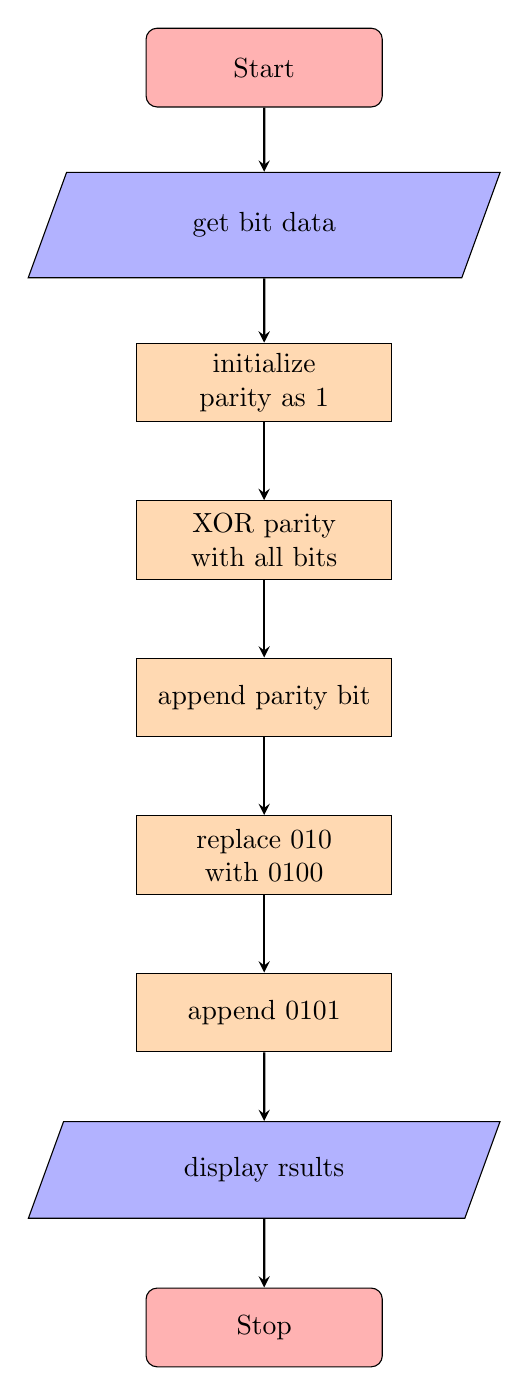
\begin{tikzpicture}[node distance=2cm]
        \node (start) [startstop] {Start};
        \node (p1) [io,below of=start] {get bit data};
        \node (p2) [process,below of=p1] {initialize parity as 1};
        \node (p3) [process,below of=p2] {XOR parity with all bits};
        \node (p4) [process,below of=p3] {append parity bit};
        \node (p5) [process,below of=p4] {replace 010 with 0100};
        \node (p6) [process,below of=p5] {append 0101};
        \node (p7) [io,below of=p6] {display rsults};
        \node (stop) [startstop,below of=p7] {Stop};

    
        \draw [arrow] (start) -- (p1);
        \draw [arrow] (p1) -- (p2);
        \draw [arrow] (p2) -- (p3);
        \draw [arrow] (p3) -- (p4);
        \draw [arrow] (p4) -- (p5);
        \draw [arrow] (p5) -- (p6);
        \draw [arrow] (p6) -- (p7);
        \draw [arrow] (p7) -- (stop);
    
    
    
    \end{tikzpicture}
    \pagebreak
    \subsection{PS1 Solution-Code}
    \verbatiminput{ps1.py}
    
    % \pagebreak
    \subsection{PS1 Output Screenshots}
    \begin{center}     
        \includegraphics[width=1.1\textwidth]{./images/ps1_001.png}
    \end{center}
    \pagebreak
    \section{Problem Satement 2}
    \textbf{3X3 Numeric Tic-Tac-Toe} (Use numbers 1 to 9 instead of X’s and O’s)
    \\One player plays with the odd numbers (1, 3, 5, 7, 9) and the other player plays with the even numbers (2,4,6,8). All numbers can be used only once. The player who puts down 15 points in a line wins (sum of 3 numbers). Always Player with odd numbers starts the game. Once a line contains two numbers whose sum is 15 or greater, there is no way to complete that line, although filling in the remaining cells might be necessary to complete a different line.
    \\Note – Line can be horizontal, vertical or diagonal\\

    \subsection{Constraints}
    $1<=Position<=9$
    \\$1<=Number<=9$
 
    \subsection{Terminal}
    \begin{itemize}
        \item Print ‘Welcome to the Game!’.	
        \item Print whether it is Player 1’s or Player 2’s chance.
        \item Get the position and number to be entered from the user.
        \item Show tic tac toe with data.
        \item Continue till the game gets draw or some player wins and show the result.
        \item Ask the user whether to continue for the next game or exit.
    \end{itemize}
    \subsection{Sample Output:}
    Welcome to the Game!\\
    Player 1’s chance\\
    Enter the position and number to be entered: 5,3\\ \\
    \includegraphics[width=.2\textwidth]{./images/ps1_ps_001.png}
    \\Player 2’s chance\\
    Enter the position and number to be entered: 7,4\\ \\
    \includegraphics[width=.2\textwidth]{./images/ps1_ps_002.png}

    ... Continue till game ends\\
    Note – Must use at least one User Defined Function.


    \subsection{PS2 algorithm}
    \begin{itemize}
        \item Save all possible lines to a 2D list lines
        \item make two 1D lists to store the board and the inputs already entered
        \item show the menu for the apropriate player
        \item receive players input
        \item check whether input is valid
        \item check whether game is over or is a draw
        \item if game is over, check if players wnat to play a new game
    \end{itemize}
    \subsection{PS2 Flow Chart}
    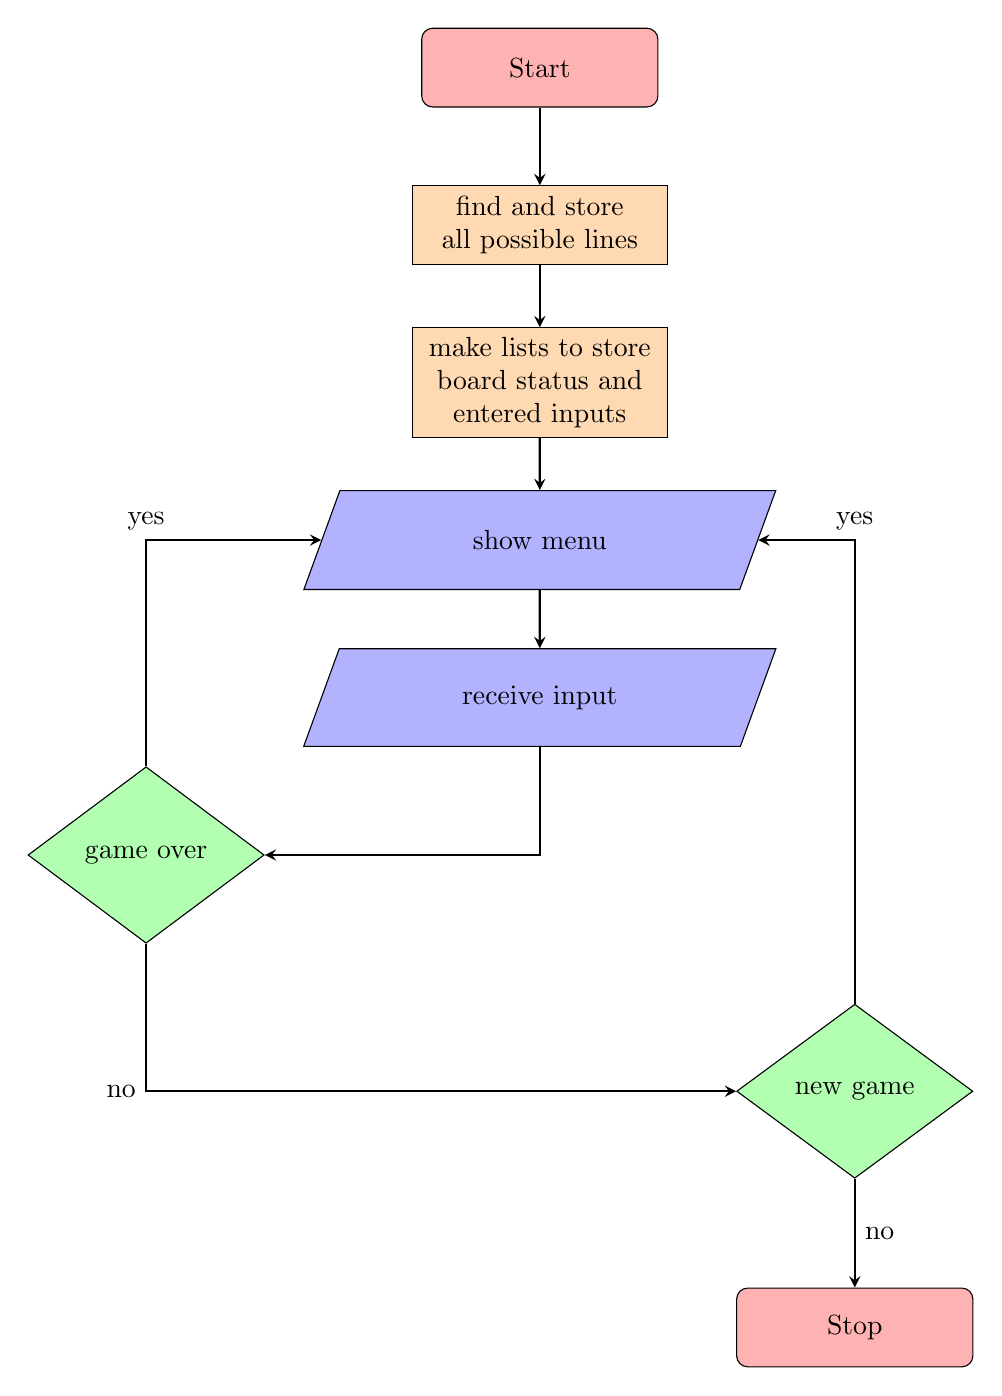
\begin{tikzpicture}[node distance=2cm]
        \node (start) [startstop] {Start};
        \node (p1) [process,below of=start] {find and store all possible lines};
        \node (p2) [process,below of=p1] {make lists to store board status and entered inputs};
        \node (p3) [io,below of=p2] {show menu};
        \node (p4) [io,below of=p3] {receive input};
        \node (p5) [decision,below of=p4,xshift=-5cm] {game over};
        \node (p6) [decision,right of=p5,xshift=7cm,yshift=-3cm] {new game};
        \node (stop) [startstop,below of=p6,yshift=-1cm] {Stop};

    
        \draw [arrow] (start) -- (p1);
        \draw [arrow] (p1) -- (p2);
        \draw [arrow] (p2) -- (p3);
        \draw [arrow] (p3) -- (p4);
        \draw [arrow] (p4) |- (p5);
        \draw [arrow] (p5) |- node[anchor=east]{no} (p6);
        \draw [arrow] (p6) |- node[anchor=south]{yes} (p3);
        \draw [arrow] (p5) |- node[anchor=south]{yes} (p3);
        \draw [arrow] (p6) -- node[anchor=west]{no} (stop);
    
    
    
    \end{tikzpicture}
    \pagebreak
    \subsection{PS2 Solution-Code}
    \verbatiminput{ps2.py}
    \subsection{PS2 Output Screenshots}
    \includegraphics[width=1.2\textwidth]{./images/ps2_001.png}
    \includegraphics[width=1.2\textwidth]{./images/ps2_002.png}
    \includegraphics[width=1.2\textwidth]{./images/ps2_003.png}
    % \pagebreak
    \section{makefile}
    \subsection{makefile code}
    \verbatiminput{makefile}
    % \subsection{makefile Screenshots}
    % \includegraphics[width=1.2\textwidth]{./images/mk_001.png}
    \subsection{makefile output}
    input : make ps1\\
    \includegraphics[width=1.2\textwidth]{./images/mk_001.png}
    input : make ps2\\
    \includegraphics[width=1.2\textwidth]{./images/mk_002.png}

    \newpage

    \section{Git and Github}
    \subsection{Github Account}
    Github Account Link : $https://github.com/2018EET2865/Assignment_8.git$
    \subsection{Git/Github  Screenshots}
    \includegraphics[width=1.2\textwidth]{./images/gt_001.png}
    \includegraphics[width=1.2\textwidth]{./images/gt_002.png}
    \includegraphics[width=1.2\textwidth]{./images/gt_003.png}

    % \newpage
	\begin{thebibliography}{9}
        \bibitem{tutor} 
        Tutorialspoint python\\
        \textit{https://tutorialspoint.com/python/index.html}
        \newline
        \bibitem{atlassian} 
        Atlassian Git tutorial \\
        \textit{https://www.atlassian.com/git/tutorials/} 
    \end{thebibliography}
    \addcontentsline{toc}{section}{References}
    \end{document}